\documentclass[12pt, a4paper]{article}
\addtolength{\oddsidemargin}{-.875in}
\addtolength{\evensidemargin}{-.875in}
\addtolength{\textwidth}{1.75in}
\addtolength{\topmargin}{-.875in}
\addtolength{\textheight}{1.75in}

\usepackage{indentfirst}
\usepackage{graphicx}
\usepackage{amsmath}


\begin{document}
\noindent
Nicholas Garrett\\ \\
Professor Fouda\\ \\
CS 4461\\ \\
2/5/2022\\ \\


\begin{center}
	\centering{	Homework 1\\ }
\end{center}

\noindent
Chapter 7\\

7.1

SJF:

\(T_{turnarround} = 200 + 400 + 600 = 1200\)\\

\(T_{response} = 0 + 200 + 400 =600\)\\

FIFO:

\(T_{turnarround} = 200 + 400 + 600 = 1200\)\\

\(T_{response} = 0 + 200 + 400 =600\)\\ \\ \\

7.2

SJF:

\(T_{turnarround} = 100 + 300 + 600 = 700\)\\

\(T_{response} = 0 + 100 + 300 =400\)\\

FIFO:

\(T_{turnarround} = 100 + 300 + 600 = 700\)\\

\(T_{response} = 0 + 100 + 300 = 400\)\\ \\ \\

7.3

RR:

\(T_{turnarround} = 100 + 300 + 600 = 700\)\\

\(T_{response} = 1 + 2 + 3 =6\)\\ \\ \\

7.4

SJF and FIFO give the same turnaround times in cases where they execute processes in the same order.\\ \\ \\

7.5

In the instances where the RR's scheduler, the timing where the cycling speed is the same as the time needed by the processes would cause RR and SJF to have the same response times.\\ \\ \\

7.6

The response time of the Shortest Job First method increases as job lengths increase. Though, the response time is the sum of the min\(\rightarrow\)max ordered operating times with the exception of the largest process time. 

Below is an example from the simulator program which shows this: \\ 

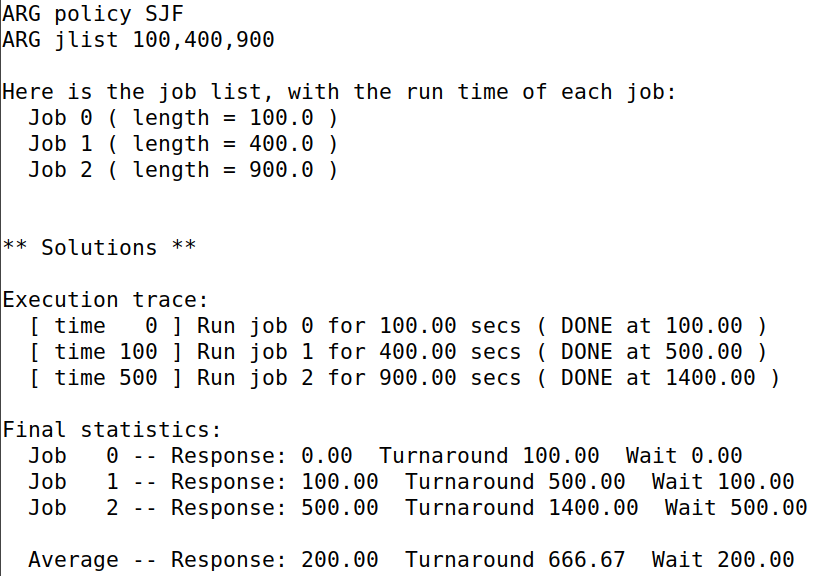
\includegraphics[height=7cm]{hw2_7_6.png} \\ \\ \\

7.7 \\ \\ \\

\noindent
Chapter 8\\

8.1

For the tasks shown below and with a quantum time of 10...

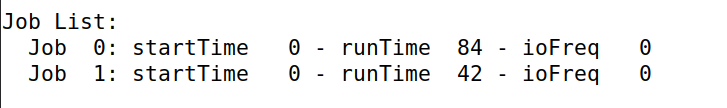
\includegraphics[width=7cm]{hw2_8_1.png} 

I would expect the execution trace to be as follows:

 \begin{center}
\begin{tabular}{ |c|c|c|} 
 \hline
 time:& Task 1 & Task 2 \\ 
 \hline
 0 & 1 & 0 \\ 
 10 & 0 & 1 \\
 20 & 1  & 0\\
 30 &0 &1 \\
 40 &1 &0\\
 50 & 0& 1\\
 60 & 1& 0\\
 70 & 0& 1\\
 80 & 1& 0\\
 90 & 0&1 \\
 100 &1 & 0\\
 110 & 0& 1\\
 120 &1 &0\\ 
 130 &0 &1 \\
 \hline
\end{tabular}
\end{center}
.\\ \\

8.2

What I would do for each of the three examples is described below: \\

Example1
Set quantum time to 10 ms, and set one operations starting at t=0 and running for 200 ms\\

Example2
Set quantum time to 10 ms, and set two operations starting at t=0 and t=100, running for 180 and 20 ms each.\\

Example3
Set quantum time to 10 ms, and set two operations starting at t=0 and having the first job issuing an I/O request every 1ms, with the I/O heavy program running for a shorter time and the other being more CPU intensive. \\ \\ \\

8.3

Set quantum time to something, and set the boost value to the same value plus 1, so that the priority levels will be offset, to cause the system to flip-flop between programs. \\ \\ \\
 
8.4

Have two jobs of the same length, the first generates an I/O request at \(\frac{99\%}{10}\) of its execution, the I/O requests account for \(\frac{1\%}{10}\) of the execution time, so for 10 cycles  the first job should start an I/O request and maintain its priority, which will all add to 1\% of its execution time, and the second job will run once before its priority is dropped and only job one will run.

I think this will work: -q 100 0,1000,99:0,1000,0  -S -i 10 \\ \\ \\

8.5

\( 5\% = \frac{1}{20} \Rightarrow \frac{1}{20} * Frequency = 10ms  \Rightarrow Frequency = 200 ms.\) The frequency to boost processes would be 200-10 ms, so 190 ms. \\ \\ \\

8.6\\ \\ \\



\noindent
Chapter 9\\

9.1

For a random seed of 1, I got the return:
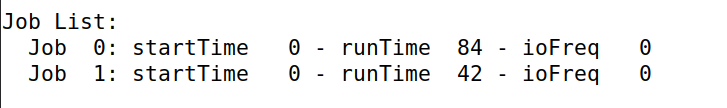
\includegraphics[width=7cm]{hw2_8_1.png} \\ 

For the first random seed, instead of incrementing for the two ticket values to get to... 495435, I took the sum of the two ticket values and found the modulus of it and 495435, which was 30. Therefore, process 0 ran first and was able to complete its tasks, and as process 1 was the only remaining process, it won all the other lotteries. \\

For the random seed of 2, I got the return:\\
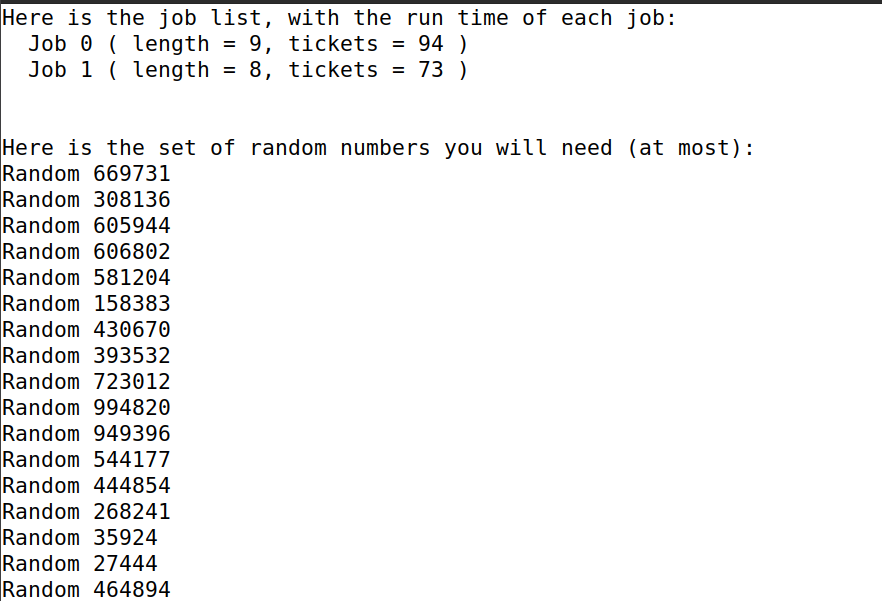
\includegraphics[width=7cm]{hw2_9_1_b.png} \\

Using the same method for calculating the winners as was used for the seed of 1, I found that process 0 ran first. The winners are shown below.
 \begin{center}
\begin{tabular}{ |c|} 
 \hline
winner: \\ 
 \hline
0 \\ 
0 \\
0\\
0\\ 
0\\
0\\
1 \\
0\\
0\\
0\\
1\\
1\\
1\\
1\\
1\\
1\\
1\\
 \hline
\end{tabular}
\end{center}
.\\ \\

Finally, for random seed 2, I got the return: \\
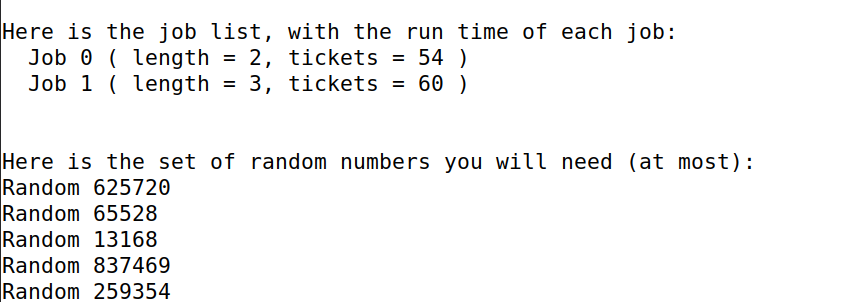
\includegraphics[width=7cm]{hw2_9_1_c.png} \\

Using the same method as the other two, I determined the order was: 
1,1,1,0,0,0\\ \\ \\

9.2

This job configuration leads to the job with more tickets being about 99\% more likely to be called first. As to whether process 0 running before process 1 completes, it really depends on the quantum time before switching processes.  \\ \\ \\

9.3

Using this configuration of two equal jobs, the fairness appears to be (both mathematically and empirically) 50\%. \\ \\ \\

9.4

From a mathematical and empirical analysis, this 50/50 split of probability seems to be maintained. However, the text indicates that the fairness should decrease as q increases.\\ \\ \\

9.5

I suppose to make a version of the graph would be extremely simple to do, though the output and testing rate would have to be optimized. If it could simply be run for, say, a thousand iterations and collect the data of which process finished first, the data graph could be fairly effective.

With a stride scheduler, as it is supposed to be more fair on shorter time scales, so it would probably start very close to fair.

\end{document}  